\section{Results}
\label{sec:results}

\begin{figure}[t]
    \centering
    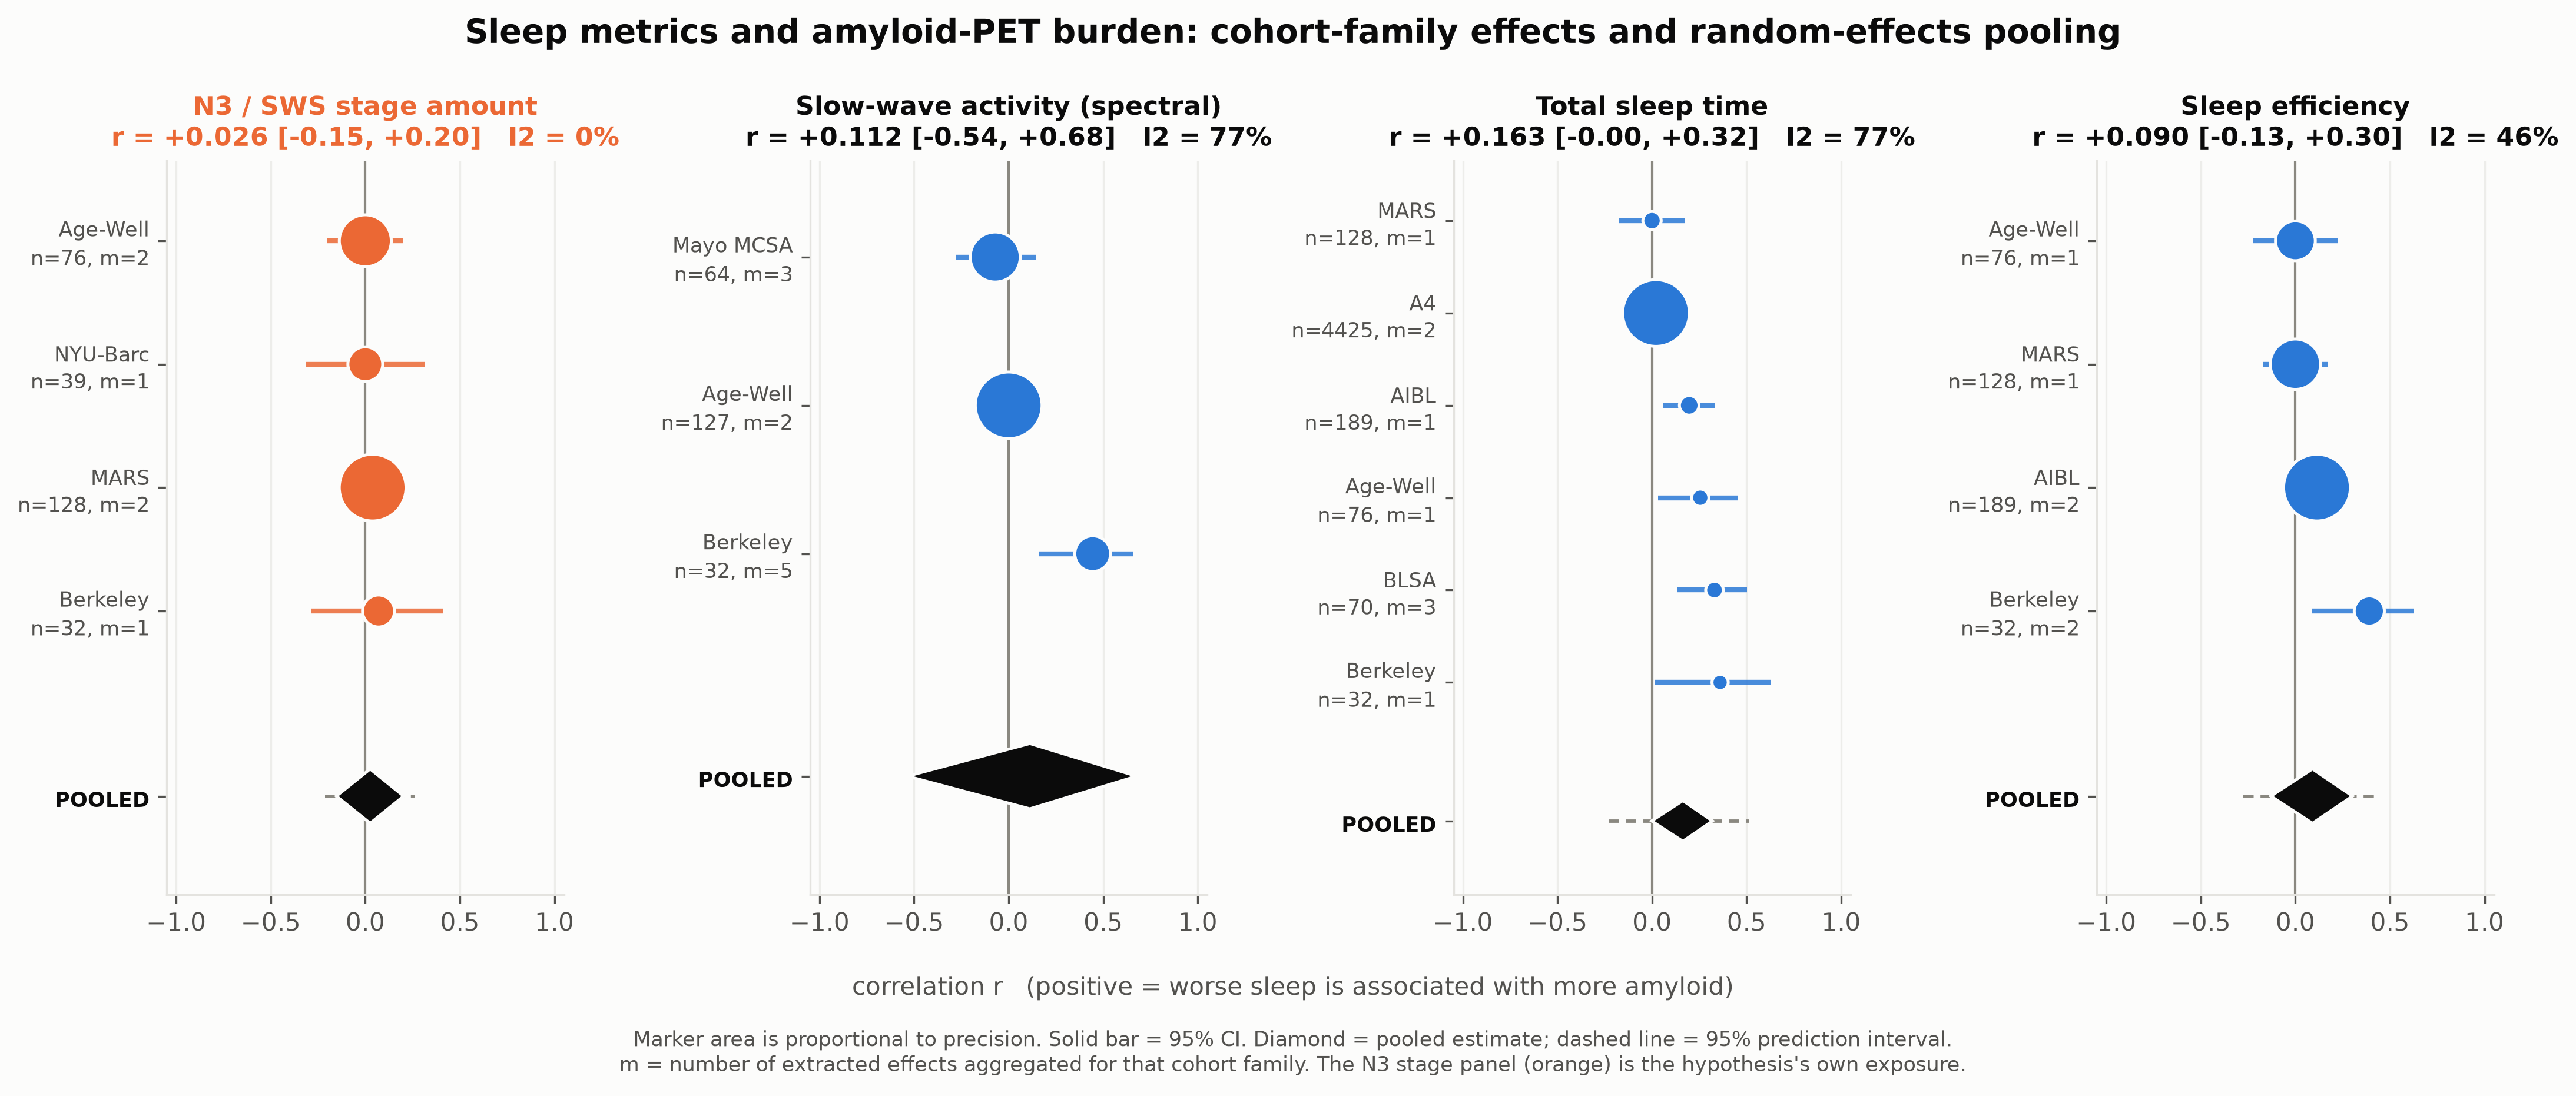
\includegraphics[width=\linewidth]{figures/fig1_forest_by_stratum.png}
    \caption{E1: cohort-family effects and random-effects pooling for the four preregistered
    exposures. Marker area is proportional to precision, solid bars are 95\% CIs, diamonds are
    pooled estimates and dashed lines are 95\% prediction intervals; $m$ is the number of
    extracted effects aggregated for that cohort family. Positive $r$ means worse sleep is
    associated with more amyloid. The hypothesis's own exposure (\stage, orange, leftmost) is the
    weakest and the most homogeneous: four independent cohort families agree there is nothing
    there. \spectral is the opposite case --- \berkeley at $r = +0.44$ against \mayo at $-0.07$
    and \agewell at $0.00$.}
    \label{fig:forest}
\end{figure}

\begin{table}[t]
    \centering
    \resizebox{\ifdim\width>\textwidth\textwidth\else\width\fi}{!}{%
    \begin{tabular}{@{}lccrcccccc@{}}
        \toprule
        \textbf{Exposure} & \textbf{$k$ eff.} & \textbf{cohorts} & \textbf{$\Sigma n$} &
        \textbf{pooled $r$} & \textbf{95\% CI} & \textbf{$p$} & \textbf{perm.\ $p$} &
        \textbf{$\tau^2$} & \textbf{$I^2$} \\
        \midrule
        \stage \textit{(the hypothesis's exposure)} & 6 & 4 & 275 & $\mathbf{+0.026}$ & $[-0.153, +0.203]$ & 0.68 & 0.50 & 0.000 & \phantom{0}0\% \\
        \spectral                                   & 10 & 3 & 223 & $+0.112$ & $[-0.535, +0.677]$ & 0.57 & 1.00 & 0.062 & 77\% \\
        \tst                                        & 9 & 6 & 4{,}920 & $\mathbf{+0.163}$ & $[-0.002, +0.320]$ & 0.052 & 0.062 & 0.016 & 77\% \\
        \se                                         & 6 & 4 & 425 & $+0.090$ & $[-0.130, +0.302]$ & 0.28 & 0.50 & 0.003 & 46\% \\
        \midrule
        \waso                                       & 2 & 2 & 108 & $+0.109$ & $[-0.975, +0.984]$ & 0.65 & 1.00 & 0.043 & 64\% \\
        Other stages (N1/N2/REM)                    & 4 & 2 & 108 & $+0.198$ & $[-0.728, +0.868]$ & 0.26 & 0.50 & 0.000 & \phantom{0}0\% \\
        \bottomrule
    \end{tabular}%
    }
    \caption{E1: pooled associations between each sleep metric and amyloid PET burden. Positive
    $r$ means \emph{worse sleep is associated with more amyloid}, so positive supports the
    hypothesis. Estimates are REML random effects with HKSJ standard errors on one synthetic
    effect per cohort family. The exposure the hypothesis names (\stage) is the weakest of the
    four preregistered strata and the only one with zero heterogeneity; the largest estimate
    belongs to \tst, which the hypothesis predicts should be weaker. Permutation $p$-values
    enumerate all $2^k$ sign flips of the cohort-level effects.}
    \label{tab:pooled}
\end{table}


\subsection{E1: the exposure the hypothesis names is the weakest of the four}
\label{sec:e1}

\Tabref{tab:pooled} and \figref{fig:forest} give the primary estimates. The pooled association
between N3 stage amount and amyloid PET burden is $r = +0.026$ (95\% CI $-0.153$ to $+0.203$,
$p = 0.68$, permutation $p = 0.50$) across 6 effects from 4 independent cohort families. Its
heterogeneity is zero ($I^2 = 0\%$, $\tau^2 = 0.000$) and its prediction interval is tight
($-0.21$ to $+0.26$): the cohort families agree with each other. Cluster-robust variance
estimation gives essentially the same answer wherever it is interpretable --- for \tst with six
clusters, $r = 0.160$ (95\% CI $-0.002$ to $0.313$, $p = 0.052$).

The ordering is the reverse of what the hypothesis predicts. \tst is the strongest stratum at
$r = +0.163$ ($p = 0.052$) across six cohort families and $\Sigma n = 4{,}920$, and \se is
$+0.090$; both exceed the exposure that is supposed to beat them. The spectral stratum sits at
$r = +0.112$ but with $I^2 = 77\%$ and a prediction interval spanning the entire correlation
scale, which is a statement about disagreement rather than about effect size.

Our \tst estimate is a useful external check. \citet{chen2025} independently pooled sleep
quality against amyloid PET at Fisher $z = 0.153$ ($r = 0.152$, $k = 9$, $n = 10{,}132$); our
$r = 0.163$ is the same order, which is reassuring evidence that the harmonisation pipeline
produces sane numbers on a stratum where an external benchmark exists.

\subsection{E2: all three specificity contrasts point the wrong way}
\label{sec:e2}

\begin{figure}[t]
    \centering
    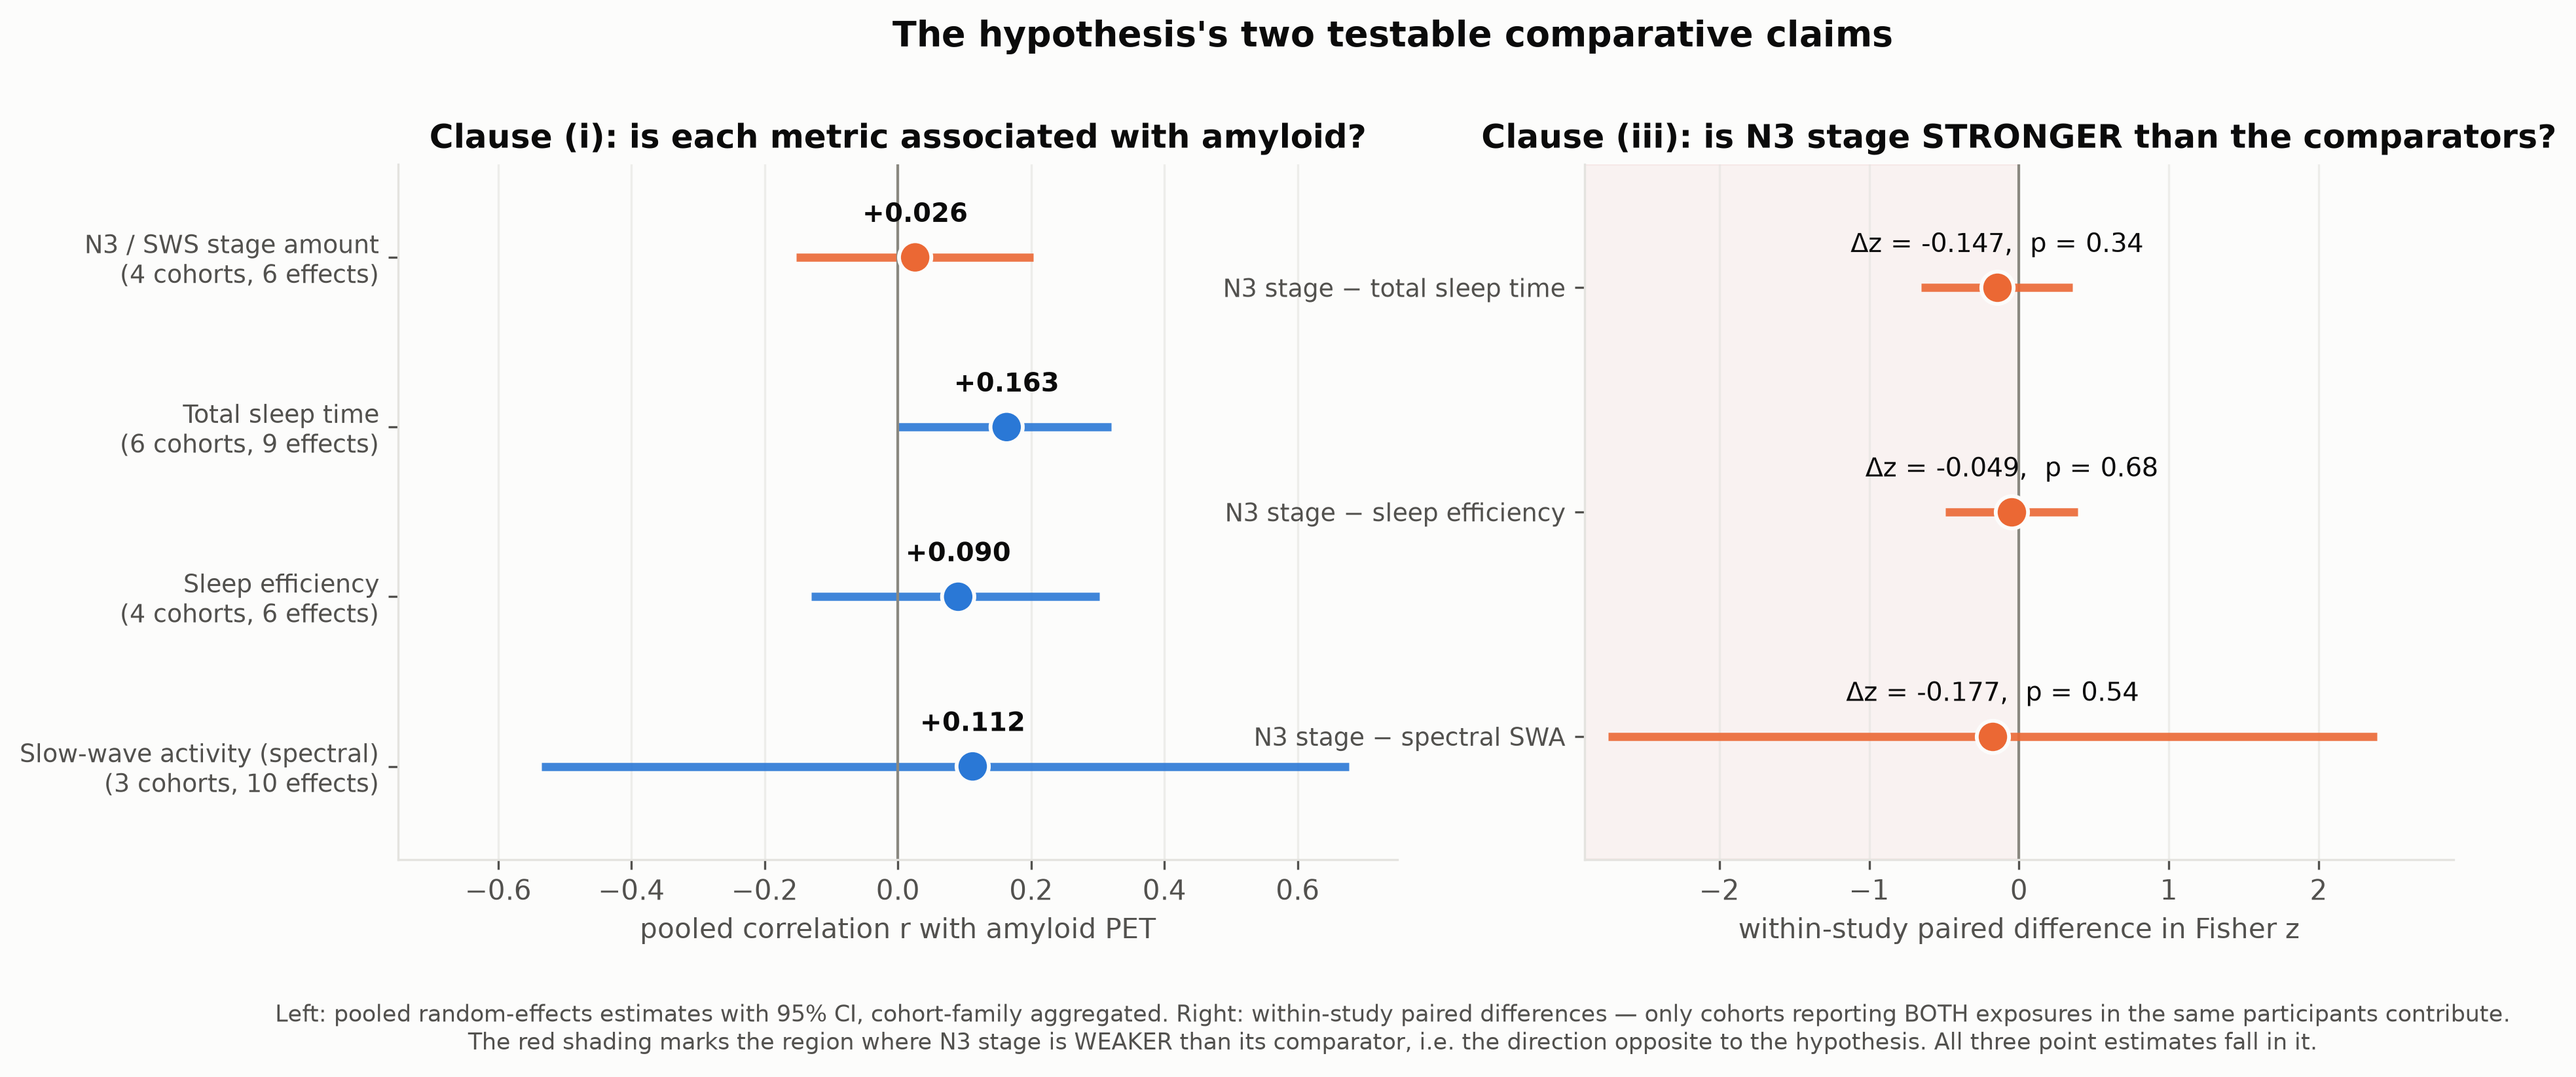
\includegraphics[width=\linewidth]{figures/fig2_specificity_contrasts.png}
    \caption{E2: the hypothesis's two testable comparative claims. \figleft{} pooled estimates with
    95\% CIs for each exposure. \figright{} within-study paired differences, where only cohort
    families reporting both exposures in the same participants contribute. Red shading marks the
    region in which \stage is \emph{weaker} than its comparator, \ie the direction opposite to
    the hypothesis; all three point estimates fall inside it.}
    \label{fig:specificity}
\end{figure}

\begin{table}[t]
    \centering
    \small
    \begin{minipage}[t]{0.51\textwidth}
    \centering
    \resizebox{\ifdim\width>\linewidth\linewidth\else\width\fi}{!}{%
\begin{tabular}{@{}lcccc@{}}
        \toprule
        \textbf{Contrast} & \textbf{shared} & \textbf{$\Delta z$} & \textbf{95\% CI} & \textbf{Holm $p$} \\
        \midrule
        \stage $-$ \tst      & 3 & $\mathbf{-0.147}$ & $[-0.651, +0.357]$ & 1.00 \\
        \stage $-$ \se       & 3 & $\mathbf{-0.049}$ & $[-0.490, +0.392]$ & 1.00 \\
        \stage $-$ \spectral & 2 & $\mathbf{-0.177}$ & $[-2.743, +2.389]$ & 1.00 \\
        \bottomrule
    \end{tabular}%
}
    \end{minipage}
    \hfill
    \begin{minipage}[t]{0.38\textwidth}
    \centering
    \resizebox{\ifdim\width>\linewidth\linewidth\else\width\fi}{!}{%
\begin{tabular}{@{}lccc@{}}
        \toprule
        \textbf{Cohort family} & \textbf{$r_{\mathrm{N3}}$} & \textbf{$r_{\mathrm{TST}}$} & \textbf{$\Delta z$} \\
        \midrule
        \agewell \citep{montagne2026} & 0.000 & 0.255 & $-0.261$ \\
        \berkeley \citep{winer2020}   & 0.070 & 0.360 & $-0.307$ \\
        \mars \citep{jin2025}         & 0.039 & 0.000 & $+0.039$ \\
        \bottomrule
    \end{tabular}%
}
    \end{minipage}
    \caption{E2: the specificity claim (clause iii), tested as a within-study paired difference
    so that only cohorts measuring both exposures in the same participants contribute.
    \textit{Left:} all three point estimates are \emph{negative} --- \stage is weaker than every
    comparator, the direction opposite to the hypothesis --- though none is individually
    significant and none survives Holm correction. \textit{Right:} per-cohort detail for the
    primary contrast; two of three cohorts favour \tst.}
    \label{tab:specificity}
\end{table}


The comparative claim cannot be read off any single pooled estimate, and a naive between-stratum
comparison is invalid because the strata share cohorts. \Tabref{tab:specificity} therefore
reports within-study paired differences. All three point estimates are negative: \stage is
$\Delta z = -0.147$ weaker than \tst, $-0.049$ weaker than \se, and $-0.177$ weaker than
\spectral. None reaches significance and none survives Holm correction, so the honest statement
is that clause (iii) is \emph{not supported} and is contradicted in direction, with the
contradiction not itself individually significant at this sample size.

The per-cohort detail matters because it shows the pattern is not driven by one study. In
\agewell, N3 gives $r = 0.000$ against $0.255$ for \tst; in \berkeley, $0.070$ against $0.360$.
Only \mars marginally favours N3, and there only because its \tst effect is a reported null.
This same pattern was visible within a single sample in \citet{winer2020}, which reported
spectral $<$1\,Hz slow-wave activity at $r = -0.52$ and N3 stage duration at $r = -0.07$ in the
same 32 participants.

\subsection{E3: measurement error predicts the opposite of what we observe}
\label{sec:e3}

\begin{figure}[t]
    \centering
    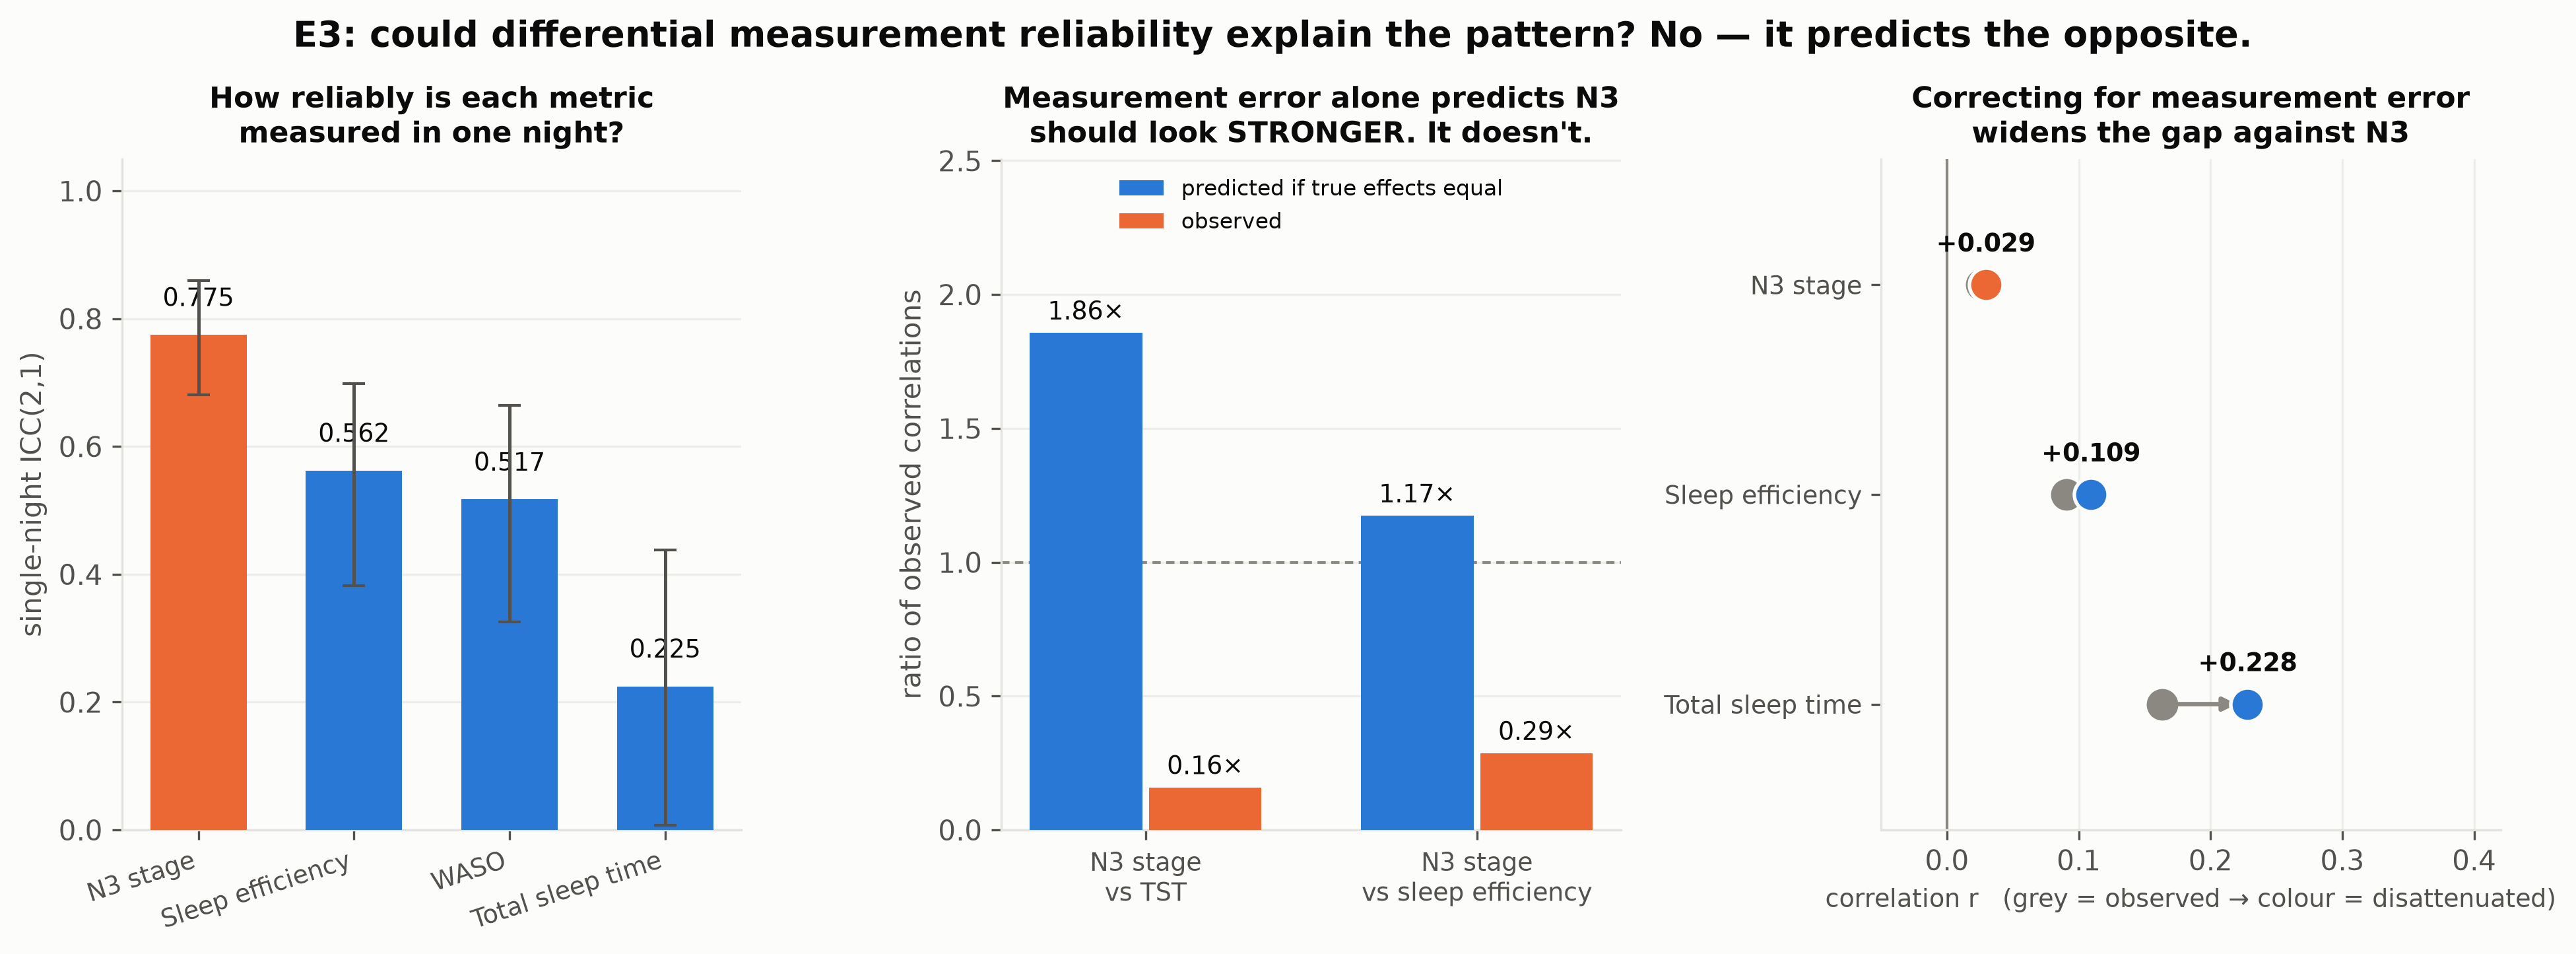
\includegraphics[width=\linewidth]{figures/fig3_reliability_null_model.png}
    \caption{E3: the measurement-reliability null model. \figleft{} empirical single-night ICC(2,1)
    per metric from 75 \sleepedf subjects with two consecutive nights each; error bars are 95\%
    CIs. \figcenter{} the ratio of observed correlations that measurement error alone predicts if
    the true correlations were identical, against the ratio actually observed. \figright{}
    correcting each stratum for its own unreliability moves \tst much further than \stage,
    widening the gap rather than closing it.}
    \label{fig:reliability}
\end{figure}

\begin{table}[t]
    \centering
    \small
    \begin{minipage}[t]{0.47\textwidth}
    \centering
    \textbf{(a) Single-night reliability and disattenuation}\\[2pt]
    \resizebox{\ifdim\width>\linewidth\linewidth\else\width\fi}{!}{%
\begin{tabular}{@{}lccc@{}}
        \toprule
        \textbf{Metric} & \textbf{ICC(2,1)} & \textbf{obs.\ $r$} & \textbf{true $r$} \\
        \midrule
        \stage & $\mathbf{0.775}$ & $+0.026$ & $\mathbf{+0.029}$ \\
        \se    & $0.562$ & $+0.090$ & $+0.109$ \\
        \waso  & $0.517$ & $+0.109$ & $+0.144$ \\
        \tst   & $\mathbf{0.225}$ & $+0.163$ & $\mathbf{+0.228}$ \\
        \bottomrule
    \end{tabular}%
}
    \end{minipage}
    \hfill
    \begin{minipage}[t]{0.44\textwidth}
    \centering
    \textbf{(b) The measurement-only prediction}\\[2pt]
    \resizebox{\ifdim\width>\linewidth\linewidth\else\width\fi}{!}{%
\begin{tabular}{@{}lccc@{}}
        \toprule
        \textbf{Ratio} & \textbf{predicted} & \textbf{observed} & \textbf{obs./pred.} \\
        \midrule
        \stage $\div$ \tst & $\mathbf{1.86\times}$ & $\mathbf{0.16\times}$ & $0.09$ \\
        \stage $\div$ \se  & $1.17\times$ & $0.29\times$ & $0.25$ \\
        \bottomrule
    \end{tabular}%
}
    \end{minipage}
    \caption{E3: could differential measurement reliability explain the ordering? No --- it
    predicts the opposite. \textit{(a)} ICC(2,1) from 75 \sleepedf subjects with two consecutive
    nights; disattenuated (``true'') $r$ divides the observed $r$ by $\sqrt{\mathrm{ICC}}$.
    Correcting for unreliability \emph{widens} the gap against \stage
    ($+0.029$ vs.\ $+0.228$). \textit{(b)} If \stage and its comparator had identical true
    correlations with amyloid, measurement error alone would still make the observed \stage
    correlation $1.86\times$ larger than \tst's. The observed ratio is about eleven times
    smaller than that prediction.}
    \label{tab:reliability}
\end{table}


\para{Is \stage just noisier?} This is the obvious defence of the hypothesis and, as far as we
can tell, it has never been tested. It fails, and it fails in an informative direction.
\Tabref{tab:reliability}a shows that single-night polysomnography measures N3\% \emph{more}
reliably than any other metric here (ICC $= 0.775$, 95\% CI $0.68$--$0.86$) and total sleep time
\emph{least} reliably (ICC $= 0.225$, 95\% CI $0.01$--$0.43$). The wake/sleep boundary in a lab
night varies enormously between nights; the depth architecture within sleep is comparatively
stable.

Classical attenuation then gives a quantitative null model. If \stage and \tst had identical
true correlations with amyloid, the observed \stage correlation should still be
$\sqrt{0.775/0.225} = 1.86\times$ larger, purely because one night measures it better. The
observed ratio is $0.16\times$ --- about eleven times below the measurement-only prediction
(\tabref{tab:reliability}b). Correcting each exposure for its own unreliability widens the gap:
true $r = +0.029$ for \stage against $+0.228$ for \tst. For \stage to have the same true
association with amyloid as \tst, its observed single-night correlation would need to be
$r = 0.201$; it is $0.026$, a shortfall of $0.175$.

\para{Two caveats, both of which cut against the hypothesis.} Six of nine \tst effects use
self-reported habitual sleep duration, whose test--retest reliability is not the single-night
PSG ICC. Restricting to PSG-measured exposures leaves the picture unchanged (\stage $+0.026$,
\tst $+0.176$, \se $+0.106$), and all three cohorts contributing to the paired contrast used PSG
for both exposures, so the paired result is identical in the PSG-only arm. Alternatively, if
self-report is treated as a reliable trait measure ($\mathrm{ICC} \approx 0.75$), \tst needs
\emph{less} upward correction --- which makes the \stage gap even harder to attribute to
measurement error.

\subsection{E4: the dose statement, and whether the dose exists}
\label{sec:e4}

\begin{figure}[t]
    \centering
    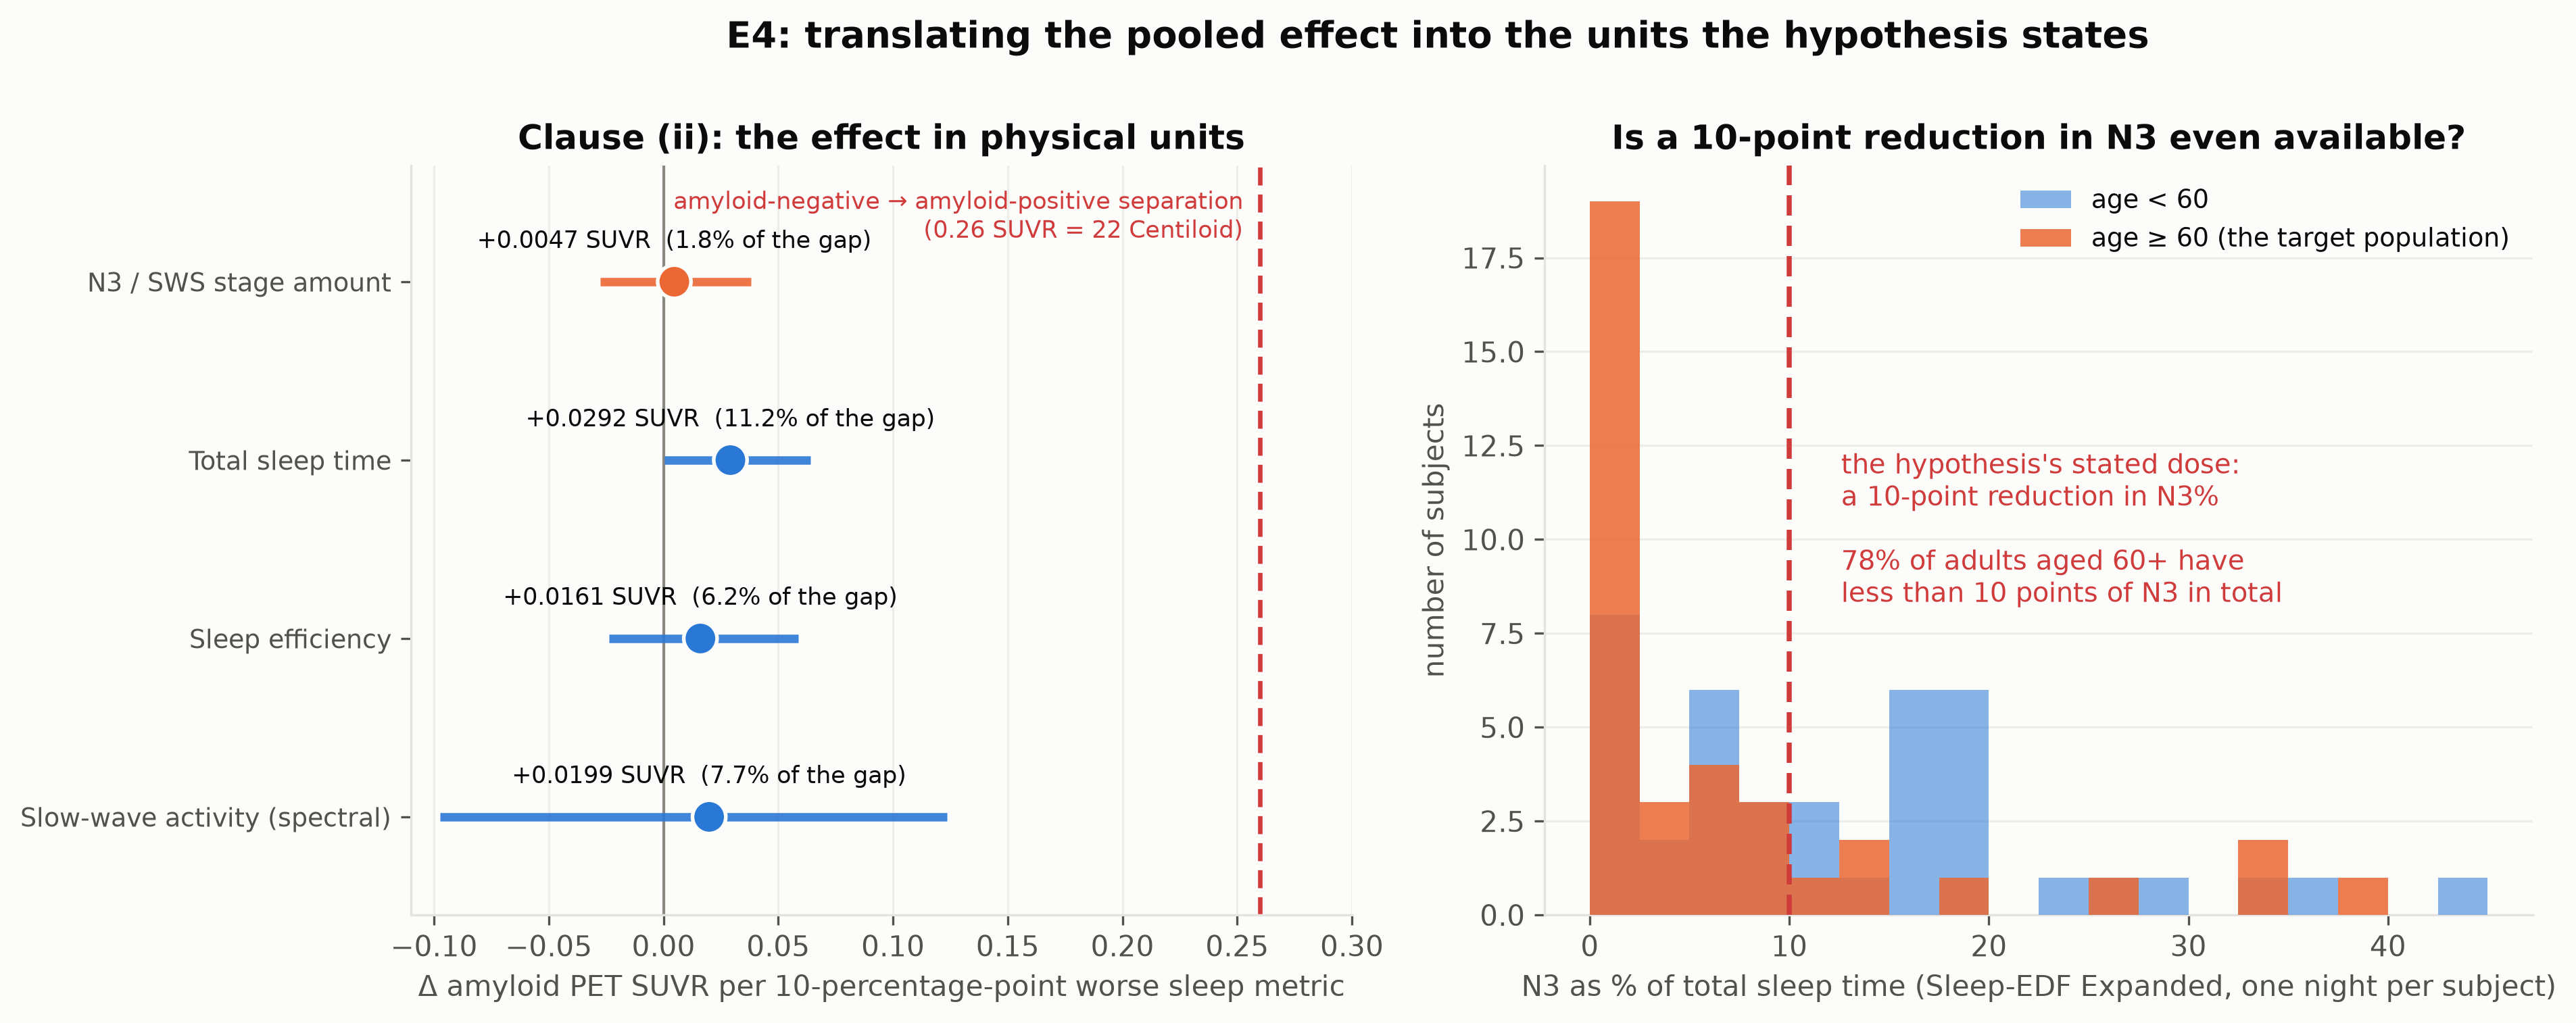
\includegraphics[width=\linewidth]{figures/fig4_dose_response_and_feasibility.png}
    \caption{E4: translating the pooled effect into the units the hypothesis states. \figleft{}
    amyloid change per 10-percentage-point worsening of each metric, with the
    amyloid-negative/positive separation (0.26\,SUVR $=$ 22 Centiloid) marked in red for scale.
    \figright{} the distribution of N3 as a percentage of total sleep time in \sleepedf; among
    subjects aged 60 and over --- the population the hypothesis concerns --- 78\% have less than
    10 percentage points of N3 in total, so the stated dose is not an available exposure
    contrast.}
    \label{fig:dose}
\end{figure}

\begin{table}[t]
    \centering
    \small
    \begin{tabular}{@{}lccccc@{}}
        \toprule
        \textbf{Exposure} & \textbf{$\Delta$SUVR} & \textbf{95\% CI} & \textbf{$\Delta$Centiloid}
        & \textbf{\% of A$-$/A$+$ gap} & \textbf{clause (ii)} \\
        \midrule
        \stage    & $\mathbf{+0.0047}$ & $[-0.028, +0.038]$ & $+0.38$ & $\mathbf{1.8\%}$ & refuted \\
        \tst      & $+0.0292$ & $[+0.000, +0.064]$ & $+2.41$ & $11.2\%$ & --- \\
        \se       & $+0.0161$ & $[-0.024, +0.059]$ & $+1.33$ & $6.2\%$ & --- \\
        \spectral & $+0.0199$ & $[-0.097, +0.124]$ & $+1.71$ & $7.7\%$ & --- \\
        \bottomrule
    \end{tabular}
    \caption{E4: the dose statement in physical units --- amyloid change per 10-percentage-point
    worsening of each sleep metric, with all three conversion inputs propagated by Monte Carlo
    (10{,}000 draws). The A$-$/A$+$ separation is 0.26\,SUVR (22 Centiloid) from
    \citet{jack2017}. The preregistered refutation criterion for clause (ii) was ``CI includes 0
    \emph{or} magnitude below $\sim$5\% of the gap''; the \stage estimate fails both. Rows for
    the comparators are expressed per 10 \pp only to place all strata on one axis; for those
    exposures the natural unit differs.}
    \label{tab:dose}
\end{table}


The conversion inputs are an age-weighted SD of N3\% of $10.2$ \pp (so a 10-point change is
$0.98$ SD of the exposure) and an SD of amyloid PET in cognitively unimpaired older adults of
$0.179$\,SUVR / $14.9$ Centiloid. The reconstructed scales imply 84.6 Centiloid per SUVR, which
matches the A$-$/A$+$ anchors as an internal consistency check.

\Tabref{tab:dose} gives the result. A 10-percentage-point reduction in N3 corresponds to
$\Delta\mathrm{SUVR} = +0.0047$ (95\% CI $-0.028$ to $+0.038$), which is $1.8\%$ of the
amyloid-negative/positive separation on the SUVR scale ($1.7\%$ on the Centiloid scale). The
preregistered refutation criterion for clause (ii) was ``CI includes 0, or magnitude below
$\sim$5\% of the gap''; the estimate fails both. Framed longitudinally against the empirical
accumulation rate in cognitively unimpaired adults of $2.1 \pm 5.3$ Centiloid/year
\citep{carvalho2024}, the same reduction maps to $+0.36$ Centiloid/year (95\% CI $-1.48$ to
$+2.12$), about 1.5 additional years of chronological ageing on that study's own age-equivalence
anchor. That longitudinal figure rests on a single cohort family and should be read as an
order-of-magnitude statement only.

\para{Is the stated dose even available?} Among \sleepedf subjects aged 60 and over ($n = 37$,
one night each), mean N3 is 7.1\% of total sleep time, the median is 1.9\%, 78\% already have
less than 10 percentage points of N3 in total, and 59\% have less than 5
(\figref{fig:dose}, right). An absolute 10-percentage-point reduction is therefore not an
achievable exposure contrast for most of the population the hypothesis concerns: the stated dose
spans roughly the whole observable range rather than a step within it.

\subsection{E5: the null survives every specification; the spectral signal does not}
\label{sec:e5}

\begin{figure}[t]
    \centering
    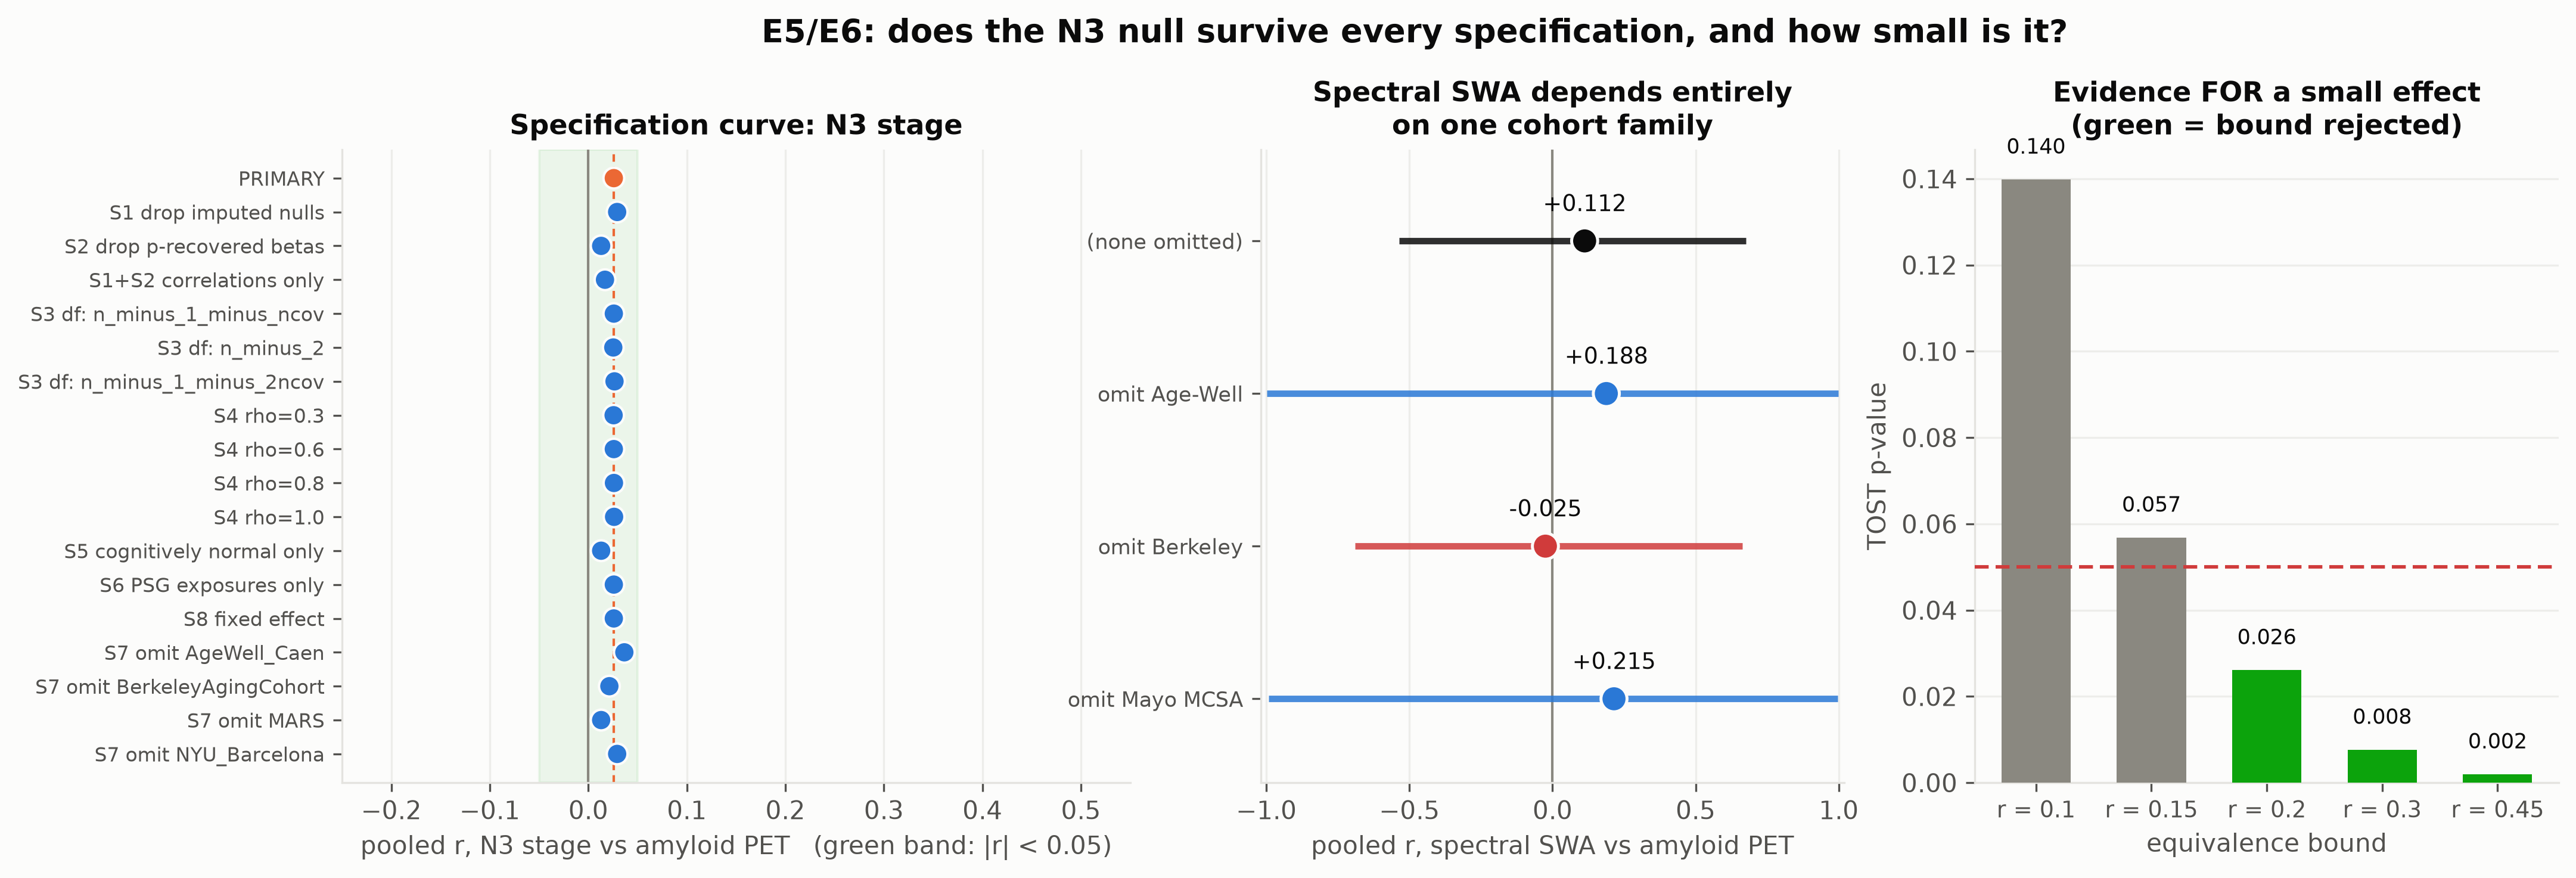
\includegraphics[width=\linewidth]{figures/fig5_robustness_and_equivalence.png}
    \caption{E5/E6: robustness and equivalence. \figleft{} specification curve for \stage across
    all 17 preregistered analyses; the green band marks $|r| < 0.05$ and every specification
    falls inside it. \figcenter{} leave-one-cohort-family-out for \spectral: removing \berkeley
    flips the pooled estimate to $-0.025$. \figright{} TOST $p$-values against five equivalence
    bounds; green bars are bounds the data reject.}
    \label{fig:robust}
\end{figure}

\begin{table}[t]
    \centering
    \small
    \begin{minipage}[t]{0.54\textwidth}
    \centering
    \textbf{(a) Specification curve (pooled $r$)}\\[2pt]
    \resizebox{\ifdim\width>\linewidth\linewidth\else\width\fi}{!}{%
\begin{tabular}{@{}lcccc@{}}
        \toprule
        \textbf{Specification} & \textbf{\stage} & \textbf{\spectral} & \textbf{\tst} & \textbf{\se} \\
        \midrule
        \textbf{PRIMARY}                 & $\mathbf{+0.026}$ & $+0.112$ & $+0.163$ & $+0.090$ \\
        S1 drop imputed nulls            & $+0.029$ & $+0.188$ & $+0.200$ & $+0.194$ \\
        S2 drop $p$-recovered betas      & $+0.013$ & $+0.215$ & $+0.151$ & $+0.036$ \\
        S1+S2 native correlations only   & $+0.017$ & $\mathbf{+0.444}$ & $+0.299$ & $+0.187$ \\
        S3 df $= n-2$                    & $+0.025$ & $+0.113$ & $+0.161$ & $+0.090$ \\
        S3 df $= n-1-2n_{\mathrm{cov}}$  & $+0.027$ & $+0.112$ & $+0.166$ & $+0.091$ \\
        S4 $\rho = 0.3$                  & $+0.026$ & $+0.122$ & $+0.167$ & $+0.104$ \\
        S4 $\rho = 0.8$                  & $+0.026$ & $+0.105$ & $+0.161$ & $+0.085$ \\
        S4 $\rho = 1.0$                  & $+0.026$ & $+0.098$ & $+0.158$ & $+0.080$ \\
        S5 cognitively normal only       & $+0.013$ & $+0.112$ & $+0.198$ & $+0.139$ \\
        S6 PSG exposures only            & $+0.026$ & $+0.112$ & $+0.176$ & $+0.106$ \\
        S8 fixed effect                  & $+0.026$ & $+0.045$ & $+0.036$ & $+0.089$ \\
        \bottomrule
    \end{tabular}%
}
    \end{minipage}
    \hfill
    \hfill
    \begin{minipage}[t]{0.40\textwidth}
    \centering
    \textbf{(b) Leave-one-cohort-family-out}\\[2pt]
    \resizebox{\ifdim\width>\linewidth\linewidth\else\width\fi}{!}{%
\begin{tabular}{@{}lcc@{}}
        \toprule
        \textbf{Omitted} & \textbf{\stage} & \textbf{\spectral} \\
        \midrule
        (none)     & $+0.026$ & $+0.112$ \\
        \agewell   & $+0.037$ & $+0.188$ \\
        \berkeley  & $+0.021$ & $\mathbf{-0.025}$ \\
        \mayo      & --- & $+0.215$ \\
        \mars      & $+0.013$ & --- \\
        NYU-Barcelona & $+0.029$ & --- \\
        \bottomrule
    \end{tabular}%
}\\[8pt]
    \textbf{(c) Small-study bias}\\[2pt]
    \resizebox{\ifdim\width>\linewidth\linewidth\else\width\fi}{!}{%
\begin{tabular}{@{}lccc@{}}
        \toprule
        \textbf{Stratum} & \textbf{$k$} & \textbf{Egger $p$} & \textbf{trim-fill} \\
        \midrule
        \stage    & 4 & 0.94 & 0 imputed \\
        \spectral & 3 & $\mathbf{0.036}$ & 0 imputed \\
        \tst      & 6 & $\mathbf{0.0035}$ & $0.163 \to 0.143$ \\
        \se       & 4 & 0.33 & 0 imputed \\
        \bottomrule
    \end{tabular}%
}
    \end{minipage}
    \caption{E5: robustness. \textit{(a)} The \stage null is invariant across all 17
    preregistered specifications (range $+0.013$ to $+0.037$). The S1+S2 row --- exactly the
    analysis a conventional meta-analysis would run --- pushes \spectral to $+0.444$, showing
    that reported nulls and $p$-recovered coefficients carry most of the corrective information.
    \textit{(b)} The \stage null holds whichever cohort family is removed; the \spectral estimate
    is carried entirely by \berkeley. \textit{(c)} Egger $p$ over all effects; with 3--6 cohort
    families these diagnostics have little power, but the detectable asymmetry sits in the
    comparator strata, not in \stage.}
    \label{tab:robustness}
\end{table}


\Tabref{tab:robustness}a shows the \stage null is invariant across all 17 preregistered
specifications, with pooled $r$ ranging only from $+0.013$ to $+0.037$. The most informative row
is S1+S2: restricted to effects reported natively as correlations --- exactly the analysis a
conventional meta-analysis would run --- the spectral estimate jumps to $r = +0.444$ and \tst to
$+0.299$. The reported nulls and $p$-recovered coefficients are precisely the evidence that
pulls the positive strata down, and precisely the evidence a conventional analysis would
discard. \stage is the one stratum unaffected either way.

Leave-one-cohort-family-out (\tabref{tab:robustness}b) tells two different stories. The \stage
null holds regardless of which family is removed ($+0.013$ to $+0.037$). The spectral estimate
does not: it falls from $+0.112$ to $\mathbf{-0.025}$ when \berkeley --- the source of
\citet{mander2015}, \citet{winer2019} and \citet{winer2020} --- is removed. The signal that
motivates the entire hypothesis is one cohort family that two independent cohorts did not
reproduce.

Small-study diagnostics (\tabref{tab:robustness}c, \figref{fig:funnel}) have almost no power at
3--6 cohort families, and we flag them as uninterpretable below $k = 5$ for Egger and $k = 10$
for trim-and-fill. But the asymmetry that \emph{is} detectable sits in the \tst
(Egger $p = 0.0035$ across effects; trim-and-fill nudges $r$ from $0.163$ to $0.143$) and
\spectral ($p = 0.036$) strata --- the comparators \stage is losing to --- not in \stage itself
($p = 0.94$). If small-study bias is inflating anything here, it is inflating the estimates the
hypothesis loses to, which makes the \stage shortfall conservative.

\subsection{E6: what this analysis could have detected}
\label{sec:e6}

\begin{table}[t]
    \centering
    \small
    \begin{minipage}[t]{0.52\textwidth}
    \centering
    \textbf{(a) What could each stratum have detected?}\\[2pt]
    \resizebox{\ifdim\width>\linewidth\linewidth\else\width\fi}{!}{%
\begin{tabular}{@{}lcccc@{}}
        \toprule
        \textbf{Stratum} & \textbf{cohorts} & \textbf{MDE $r$} & \textbf{pow.\ $r{=}0.30$} & \textbf{pow.\ $r{=}0.45$} \\
        \midrule
        \stage    & 4 & $\mathbf{0.157}$ & 1.00 & 1.00 \\
        \spectral & 3 & $0.417$ & 0.50 & 0.86 \\
        \tst      & 6 & $0.180$ & 1.00 & 1.00 \\
        \se       & 4 & $0.153$ & 1.00 & 1.00 \\
        \bottomrule
    \end{tabular}%
}
    \end{minipage}
    \hfill
    \hfill
    \begin{minipage}[t]{0.40\textwidth}
    \centering
    \textbf{(b) Equivalence tests on \stage}\\[2pt]
    \resizebox{\ifdim\width>\linewidth\linewidth\else\width\fi}{!}{%
\begin{tabular}{@{}lcc@{}}
        \toprule
        \textbf{Bound} & \textbf{$p_{\mathrm{TOST}}$} & \textbf{conclusion} \\
        \midrule
        $r = 0.10$ & 0.140 & not rejected \\
        $r = 0.15$ & 0.057 & not rejected \\
        $r = 0.20$ & $\mathbf{0.026}$ & \textbf{rejected} \\
        $r = 0.30$ & $\mathbf{0.008}$ & \textbf{rejected} \\
        $r = 0.45$ & $\mathbf{0.002}$ & \textbf{rejected} \\
        \bottomrule
    \end{tabular}%
}
    \end{minipage}
    \caption{E6: precision. \textit{(a)} Minimum detectable effect at 80\% power, computed at the
    cohort-aggregated variances and the estimated $\tau^2$. \spectral is the one stratum too
    imprecise to support a conclusion in either direction. \textit{(b)} Equivalence testing
    converts ``no evidence of an effect'' into evidence of no meaningful effect: the data are
    inconsistent with a true \stage/amyloid correlation as large as $r = 0.20$, and \emph{a
    fortiori} with the $r \approx 0.45$ effects reported for spectral slow-wave activity. They
    cannot rule out a genuinely small effect of $r \approx 0.10$--$0.15$.}
    \label{tab:precision}
\end{table}


A negative result is only informative if it states its own resolution. \Tabref{tab:precision}a
gives the minimum detectable effect at 80\% power: $r = 0.157$ for \stage, $0.180$ for \tst,
$0.153$ for \se, and $0.417$ for \spectral. Equivalence testing on \stage
(\tabref{tab:precision}b) rejects bounds of $r = 0.20$ ($p_{\mathrm{TOST}} = 0.026$), $0.30$
($p = 0.008$) and $0.45$ ($p = 0.002$), but not $0.15$ ($p = 0.057$) or $0.10$ ($p = 0.140$).
The data are therefore inconsistent with a true N3-stage/amyloid correlation as large as
$r = 0.20$, and \emph{a fortiori} with the $r \approx 0.45$ effects reported for spectral
slow-wave activity; they cannot rule out a genuinely small effect of $r \approx 0.10$--$0.15$.
For \spectral, no bound is rejected even at $r = 0.45$: that stratum's honest verdict is
\emph{insufficient evidence}, not \emph{no effect}.

\subsection{The CSF secondary analysis}
\label{sec:csf}

\begin{figure}[t]
    \centering
    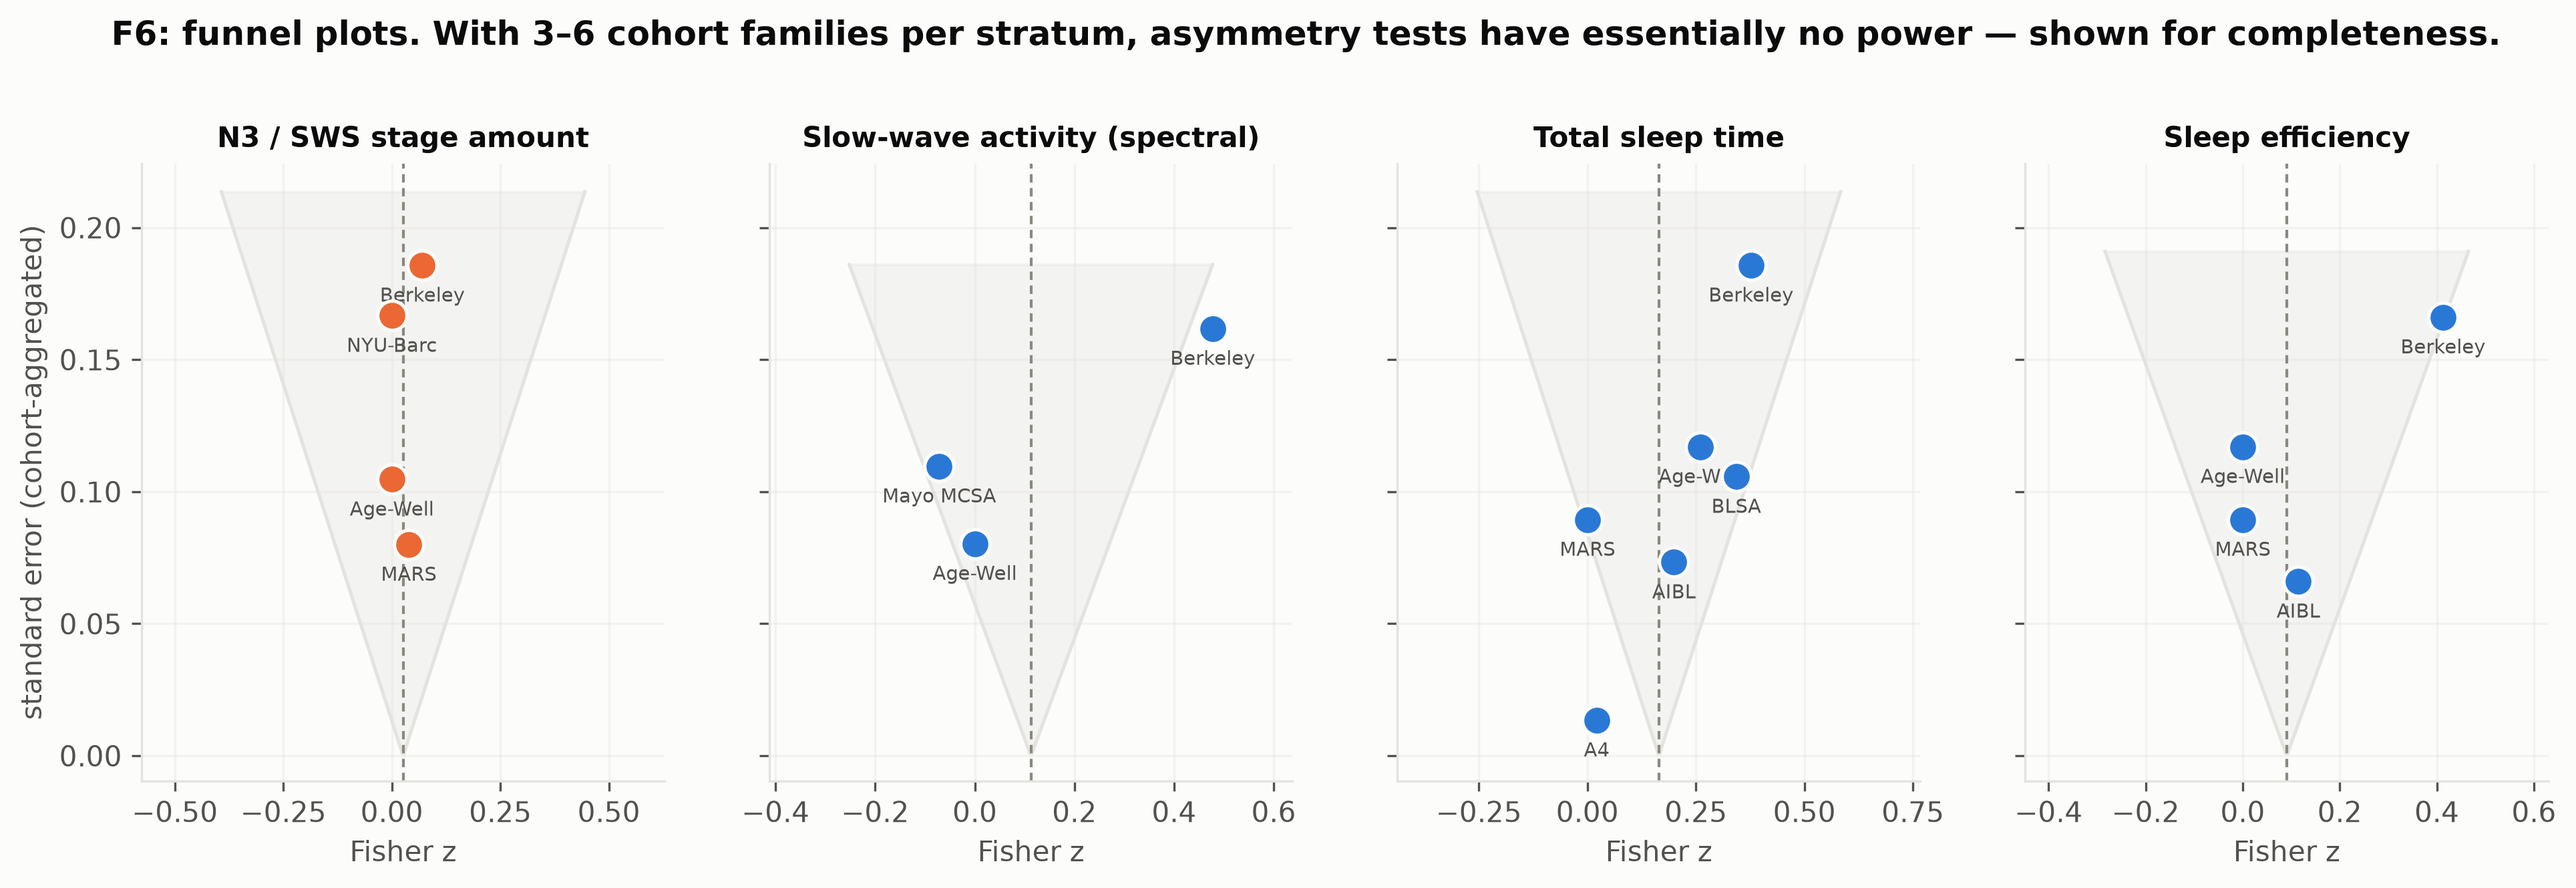
\includegraphics[width=0.92\linewidth]{figures/fig6_funnel.png}
    \caption{Funnel plots per stratum with Egger regression lines. With 3--6 cohort families
    these are near-powerless and we do not read them as evidence of publication bias; we report
    them because the only detectable asymmetry sits in the comparator strata rather than in
    \stage.}
    \label{fig:funnel}
\end{figure}

Nine CSF amyloid-beta42 effects were extracted and analysed as a cognitive-status-stratified
secondary. In cognitively normal samples \citep{varga2016,ju2017} the \stage effect is
$r = +0.355$ (95\% CI $0.066$ to $0.589$) and the spectral effect $r = +0.502$ (95\% CI $-0.862$
to $0.984$); in the mixed SCI/MCI/AD sample of \citet{liguori2020} ($n = 258$), \stage gives
$r = +0.362$, \tst $+0.306$ and \se $+0.403$. Taken at face value these look supportive, and we
report them for completeness, but they are not admissible as evidence for this hypothesis. The
outcome is soluble CSF amyloid-beta42, which inversely proxies deposited plaque and whose sign
relative to burden flips with disease stage --- which is exactly why the pre-deposition and
post-deposition samples cannot be pooled. And \citet{ju2017}, the one genuine human experiment,
measures the acute overnight production/clearance balance in 17 people, not chronic plaque
accumulation. Our result constrains the chronic-deposition claim, not the acute one.
